\section{(Basic): Explore the content of the ELM DB}
\label{sec:explore_content}

The core of the ELM database is a repository of manually annotated motifs and
instances. As of December 2016, ELM contains over 260 motif classes categorized
into 6 different types: DOC (docking), LIG (Ligand binding), DEG (degradation),
CLV (cleavage), MOD (post translational modifications), and TRG
(targeting/anchoring) motifs (Figure functional\_classification\_of\_SLiMs).
These motifs are derived from various types of experiments reported in
literature. Each manually annotated motif also has a set of bona fide instances
(occurrences) of this motif. Currently, there are over 3000 annotated instances
annotated from over 2500 publications. The motif classes and motif instances
have been uploaded by a large group of annotators from around the globe. The
complete catalogue of manually curated data can be searched, browsed and
explored on the ELM website

TODO MARC: explain: elms, annotations, classes, instances, regular expressions. And links to GO, methods PSI. we use DOC CYCLIN etc as example.

%
% Subsection: Necessary Resources
%
\subsection{Necessary Resources}
\subsubsection{Software \& Hardware}
A modern browser such as Firefox, Chrome, or Safari. ELM is best viewed
on a laptop or desktop computer, although tablets and smartphones will
also work.



%
% Subsection: Database content overview 
%
\subsection{Database content overview}
\label{subsec:explore_content_database}


% Counter for steps
\begin{enumerate}

\begin{figure}[h!]
	\centering
	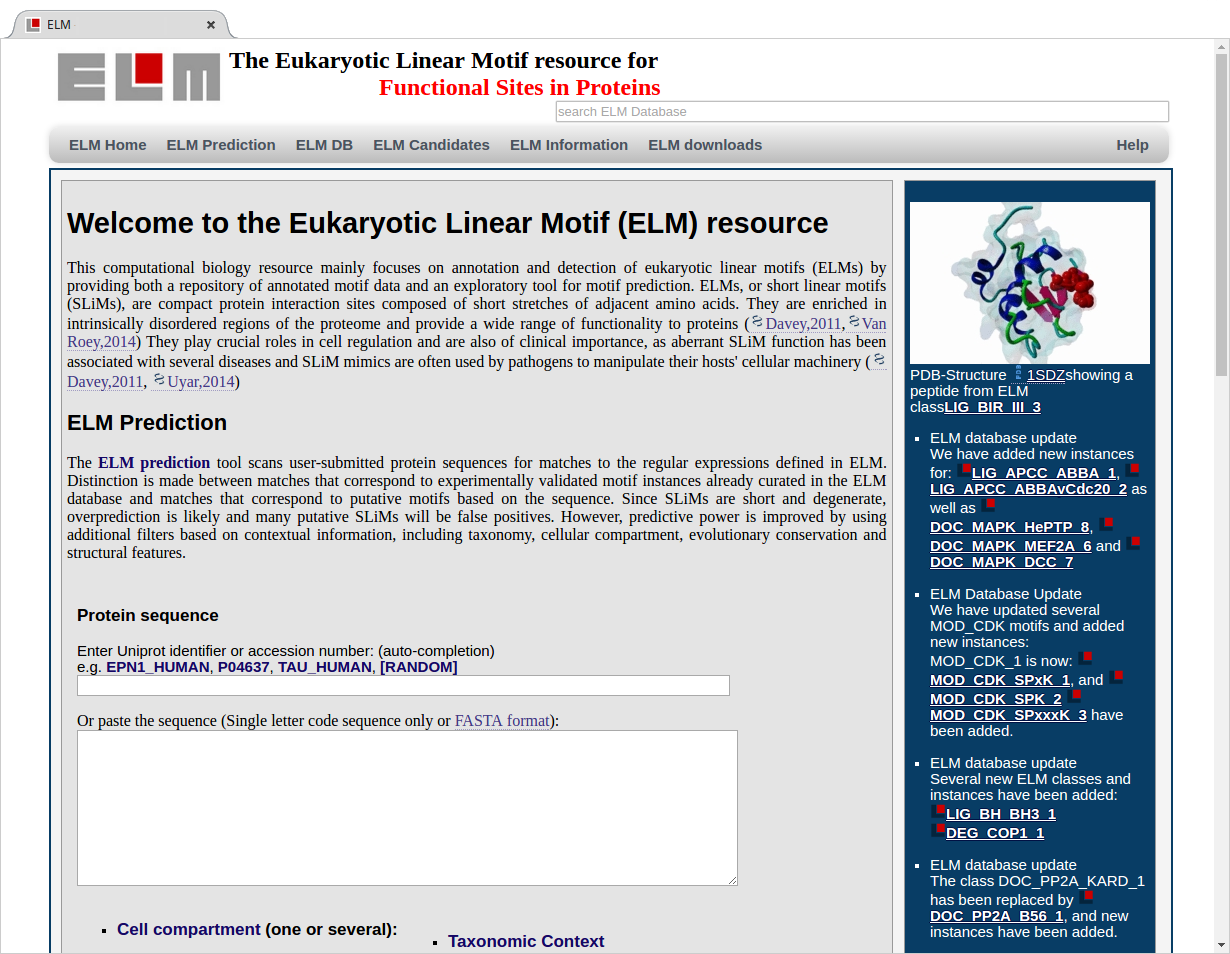
\includegraphics[width=\textwidth]{Figures/explore_content/home.png} 
	\caption{
		The homepage of the ELM database (\rurl{elm.eu.org}).
	}
	\label{fig:explore_content_home}
\end{figure}

\item The ELM database is an online web resource. Open a browser and navigate
	to \rurl{elm.eu.org} to visit the homepage
	(Fig. \ref{fig:explore_content_home}).
	This page shows a brief explanation of the ELM resource, and a form to 
	search for SLiMs (which we cover in further detail in 
	\ref{sec:predicting_p53} and \ref{sec:predicting_cv_0974}).
	The column to the right is the news column, and is continually
	updated with the latest news about changes and additions to the database. 

\begin{figure}[h!]
	\centering
	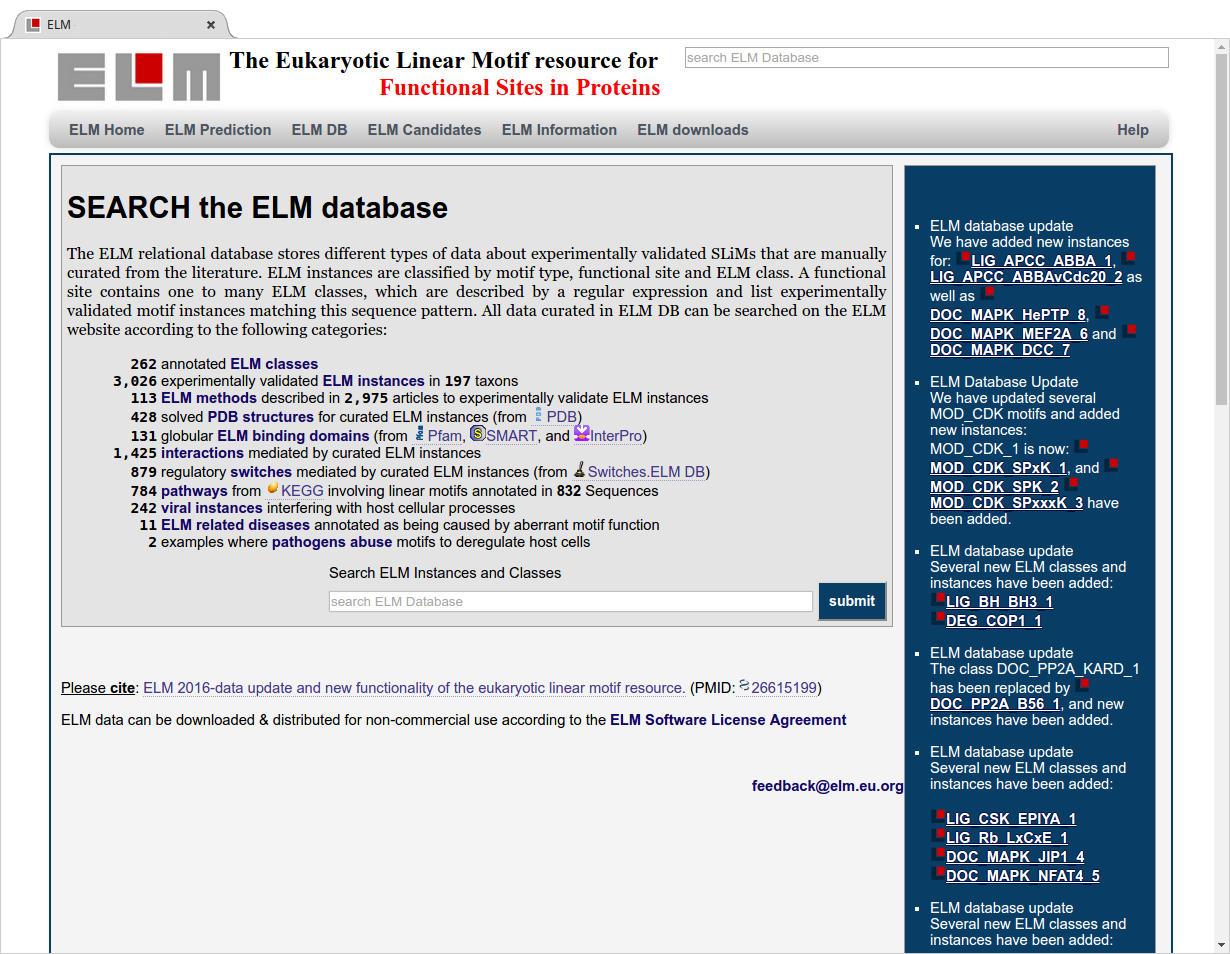
\includegraphics[width=\textwidth]{Figures/explore_content/stats.png} 
	\caption{
		The ELM database statistics overview page shows the most up to
		date database statistics. As of January 2017 ELM has just over
		3000 annotated instances in 262 different motif classes.
	}
	\label{fig:explore_content_stats}
\end{figure}

\item On the ELM homepage click on the menu link \button{ELM DB} for an overview of
	the database statistics (Fig. \ref{fig:explore_content_stats}).
	This page displays the types and amounts of annotations contained in
	the database and a few links to third-part databases.
	Each line contains at least one link which will take you
	to the corresponding contents page (for example, clicking on
	\button{ELM instances} will take you to the page displaying all of the
	annotated instances in the database).

%
% Subsection: Browsing motif classes and instances
%
\subsection{Browsing motif classes and annotated instances}
\label{subsec:explore_content_classes_and_instances}

\begin{figure}[h!]
	\centering
	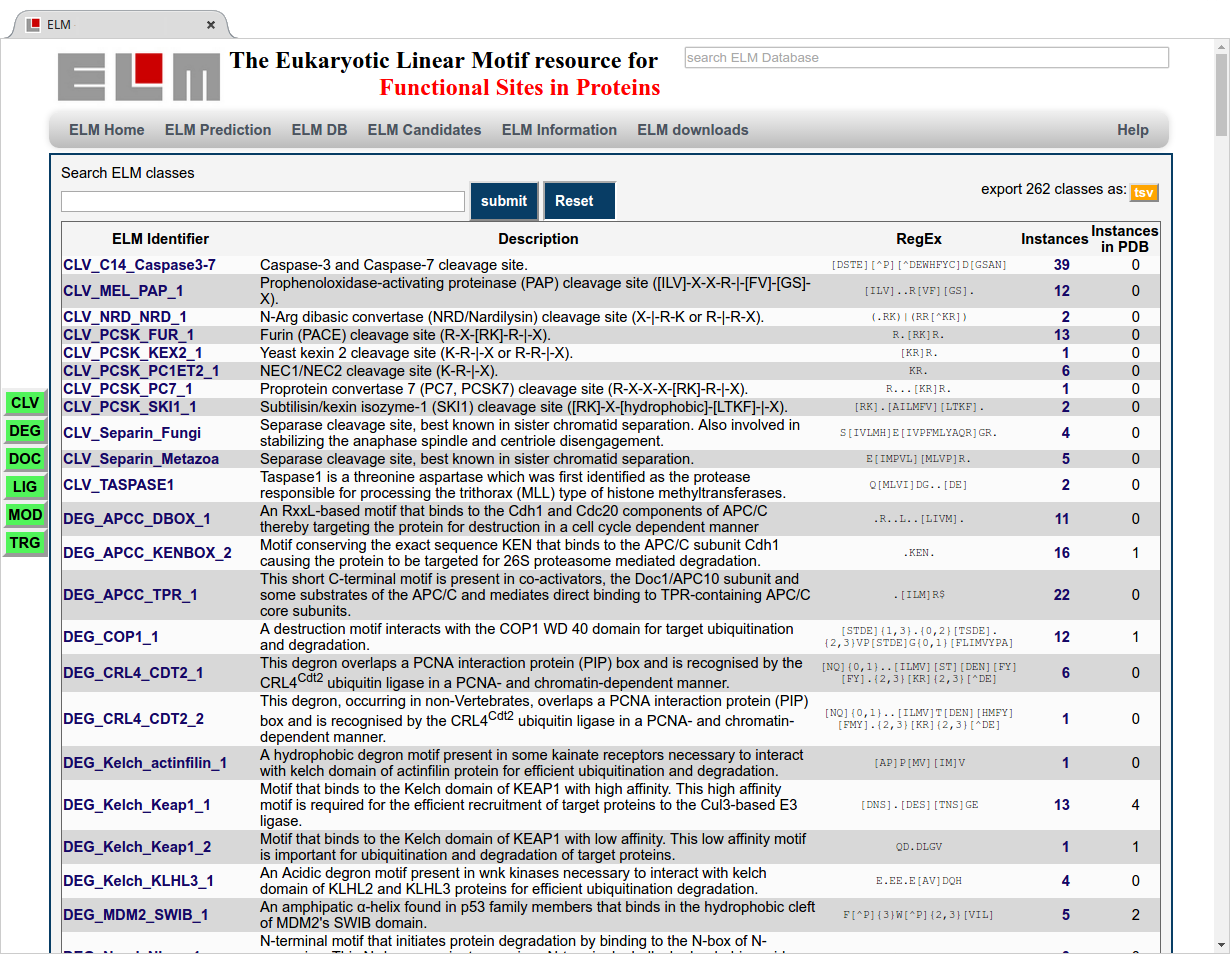
\includegraphics[width=\textwidth]{Figures/explore_content/elms.png} 
	\caption{
		The list of all motif classes annotated in the ELM database.
	}
	\label{fig:explore_content_elms}
\end{figure}

\item Click on the sub-menu \button{ELM classes} under \button{ELM DB} to visit
	the page listing all of the ELM classes
	(Fig. \ref{fig:explore_content_elms}).
	For each class, the following information is provided: ELM identifier,
	short description, regular expression, number of instances annotated
	for each class, and number of structures available. For details on each
	class, click on the ELM identifier; to get a list of annotated
	instances for an individual class, click on the number of instances.

	\sdesc{Use the search bar at the top of the page to filter for certain
		motif classes. For example, typing ``MAPK'' and hitting submit
		will perform a full-text search on all motif classes in the ELM
		database containing the term ``MAPK''. The green buttons on the
		left can also be used to filter this table. For example,
		toggling the ``DOC'' button will remove all DOC classes
		from the table (and clicking it again will bring them back).
		Lastly, the yellow \button{tsv} link can be used to export all
		motif classes as a ``tab separated values'' file.} 

\begin{figure}[h!]
	\centering
	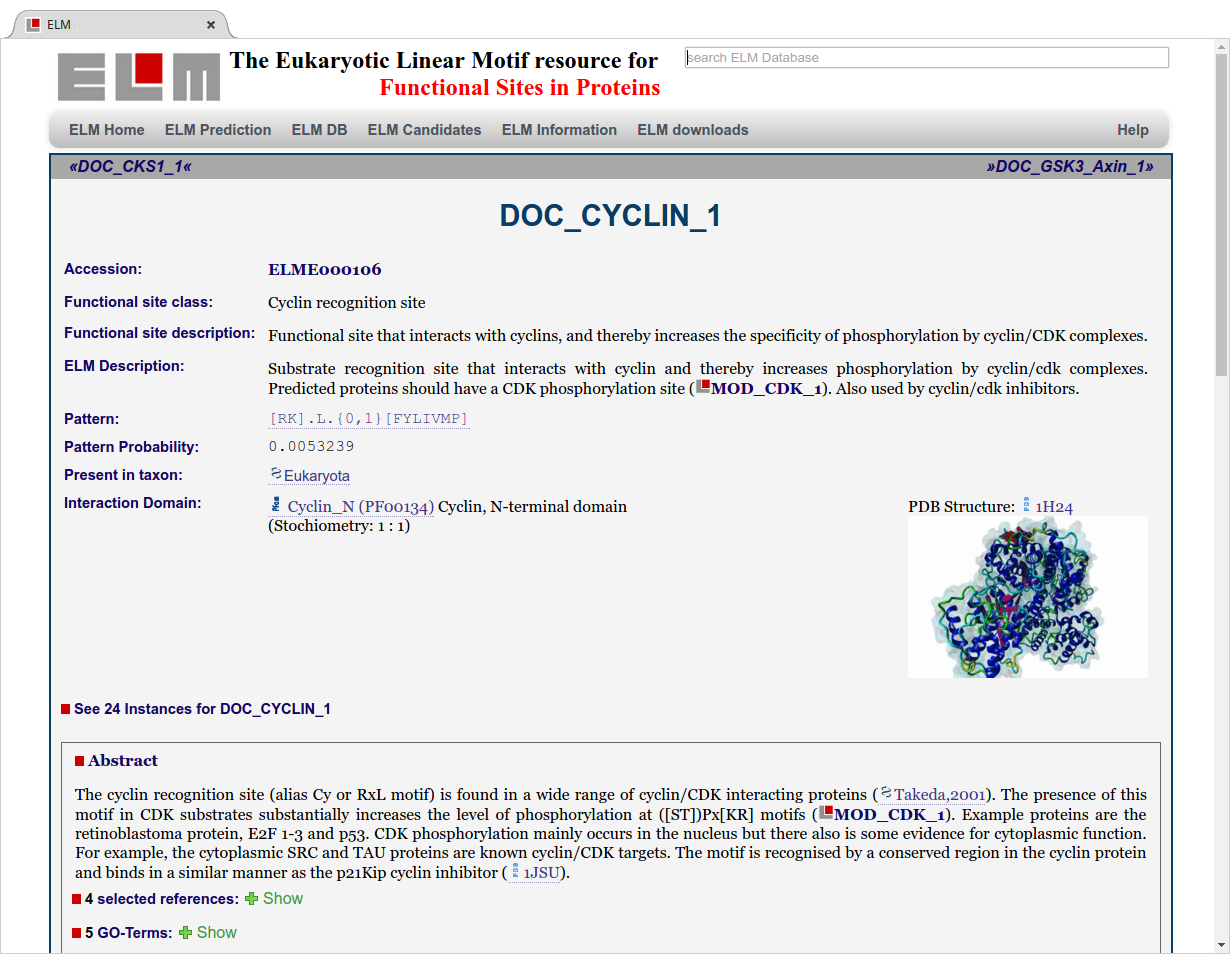
\includegraphics[width=\textwidth]{Figures/explore_content/doc_cyclin_1_class.png}
	\caption{
        The motif details page for \motif{DOC\_CYCLIN\_1}. This page
	contains all of the manual annotation details for the
    \motif{DOC\_CYCLIN\_1} motif, the biological background summarized from
	the scientific literature including links to the primary
	literature and to external resources (Pubmed \cite{27899561},
	the Gene Ontology \cite{27899567}, PDB (\cite{12037327}) and
	more).
	}
	\label{fig:explore_content_doc_cyclin}
\end{figure}

\item Search the table for the term \motif{DOC\_CYCLIN\_1} and click on 
	\button{DOC\_CYCLIN\_1} in the left column to
	navigate to the page with details about the
	\motif{DOC\_CYCLIN\_1} motif class
	(Fig. \ref{fig:explore_content_doc_cyclin}).
	This page contains a description of the
	functional site class (a Cyclin recognition site), and a short
	description of the ELM and its regular expression, as well as a
	probability score, the taxonomic distribution of the motif and which
	domain (if any) is responsible for the interaction.

	\sdesc{The probability score is the probability that the regular
		expression represents a random selection of amino acids
		(similar to an information content score). A lower score
		indicates that the motif pattern is more difficult to find by
		chance in a random sequence.}

\item Scroll further down the \motif{DOC\_CYCLIN\_1} page 
	(Fig. \ref{fig:explore_content_doc_cyclin}) to view
	more details about the manually annotated data and instances in the
	database (Fig. \ref{fig:explore_content_doc_cyclin_1_abstract_instances})
	The ``abstract'' contains a more detailed description of the motif
	annotation. Click on the \button{show} button next to the ``selected
	references'' header for a list of publications relevant to this motif.
	Click on \button{show} next to ``GO terms'' for a complete list of all
	Gene Ontology (GO) terms annotated for this motif.

\begin{figure}[h!]
	\centering
	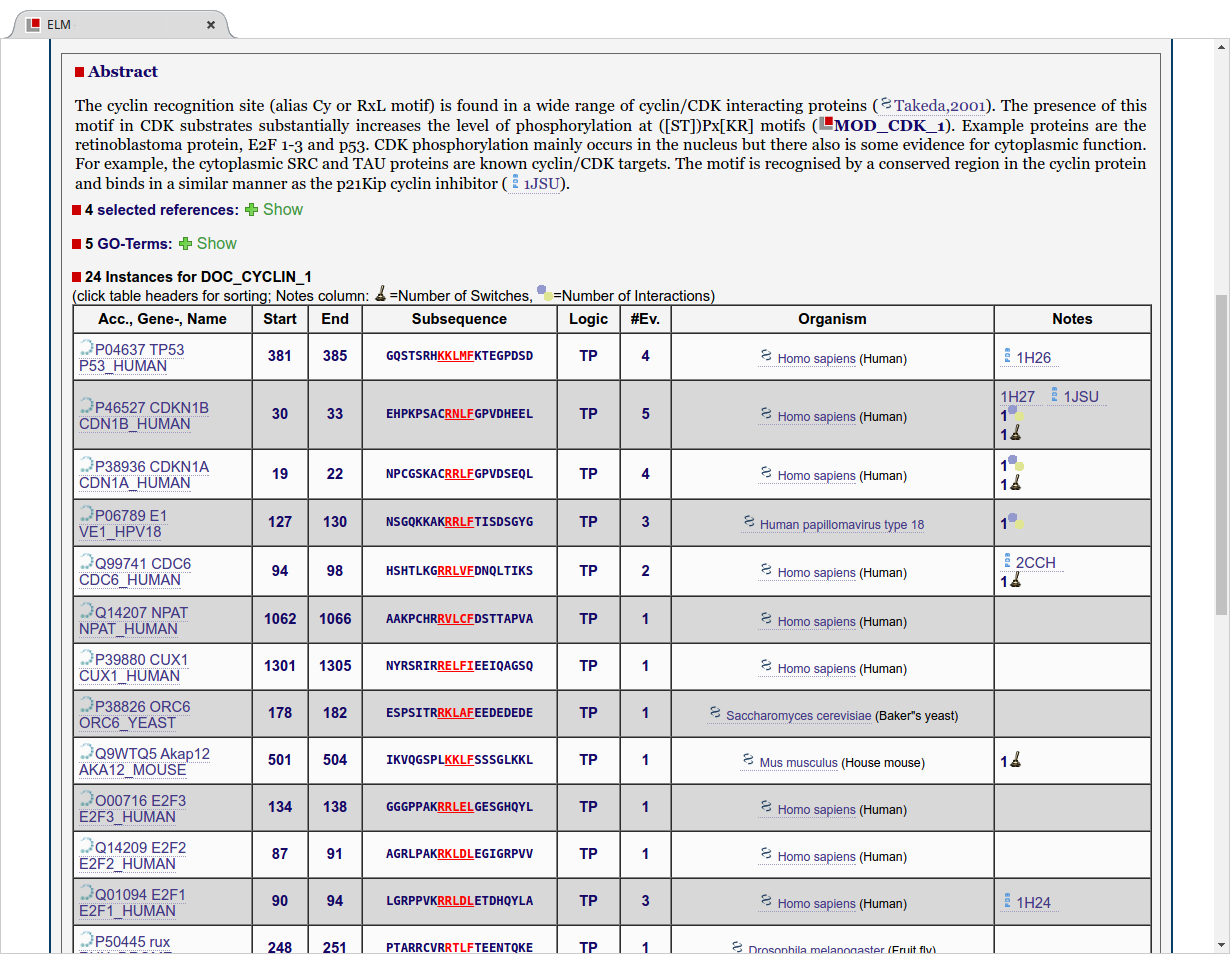
\includegraphics[width=\textwidth]{Figures/explore_content/doc_cyclin_1_abstract_instances.png}
	\caption{
		The second part of the \motif{DOC\_CYCLIN\_1} motif details page
		shows the motif abstract GO terms, and the list of annotated
		instances.
	}
	\label{fig:explore_content_doc_cyclin_1_abstract_instances}
\end{figure}

\item Scroll further down the \motif{DOC\_CYCLIN\_1} page to view
	the ``Instances'' header
	(Fig. \ref{fig:explore_content_doc_cyclin_1_abstract_instances})
	This table contains the list of all annotated \motif{DOC\_CYCLIN\_1}
	instances in the database of this motif. This includes the protein
	identifier, the start and end positions of the instance, the specific
	sequence matching the regular expression representing the motif and
	the ``logic'' of the instance.
	The ``\# Ev.'' indicates the number of experimental evidences
	associated with the annotation. ``Organism'' indicates in which  
	species in which the protein is found. Lastly the ``Notes'' column
	contains links to any ``interactions'' or ``switches'' present in the
	database, as well as links to PDB if this structure exists in PDB.

	\sdesc{The instance ``logic'' is an annotation of whether this is a
		\textit{bona-fide} instance, or whether it is a non-functional
		instance. \textit{TP} (True positive) indicates the instance is
		annotated with experimental evidence showing it is functional.
		\textit{FP} (False Positive) instances have experimental
		evidence suggesting function, but are believed to be
		non-functional after careful examination by our annotators.
		\textit{TN} (True Negative) instances have been experimentally
		determined to be non-functional, and \textit{U} (Unknown)
		instances do not have enough evidence to determine whether it
		is functional or not. The overwhelming majority of instances in
		ELM are \textit{TP}s.}


\begin{figure}[h!]
	\centering
	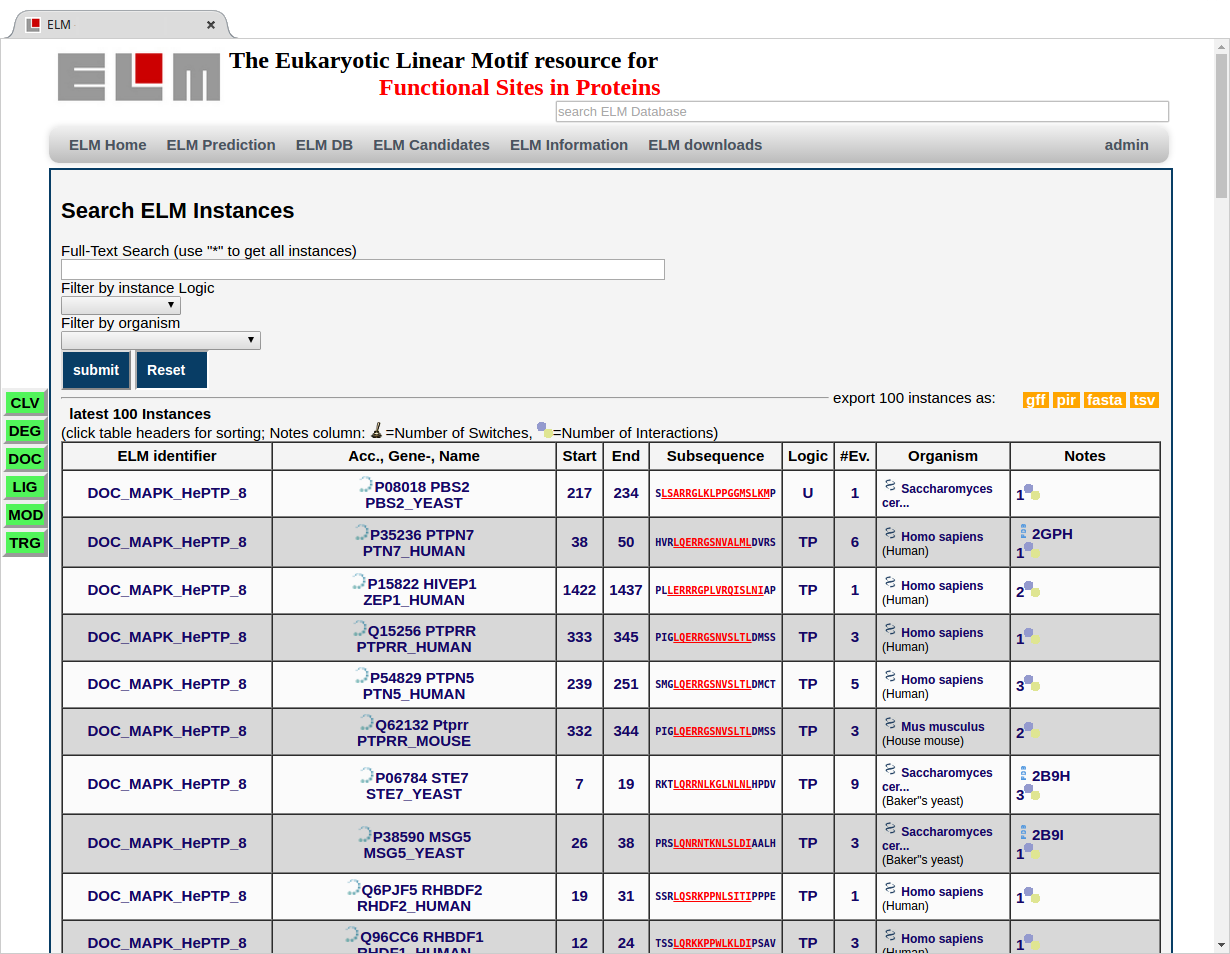
\includegraphics[width=\textwidth]{Figures/explore_content/instances.png} 
	\caption{
		The ``instances'' page can be used to search for instances in
		the ELM database. 
	}
	\label{fig:explore_content_instances}
\end{figure}

\item Click on the sub-menu \button{ELM instances} in \button{ELM DB} to visit
	the page where you can search and browse the instances annotated in ELM.
	(Fig. \ref{fig:explore_content_instances}).
	Note that only the first 100 instances matching the search criteria are shown.
	The search form can be used to filter results by a full text search, by
	instance logic, or organisms.

	\sdesc{This table can be filtered by motif class using the green toggle
		filters on the left hand side. Lastly, the yellow buttons at
		the top of the page can be used to download the instances in
		the following formats: \fileformat{gff}, \fileformat{pir},
		\fileformat{fasta} or \fileformat{tsv.}}

\begin{figure}[h!]
	\centering
	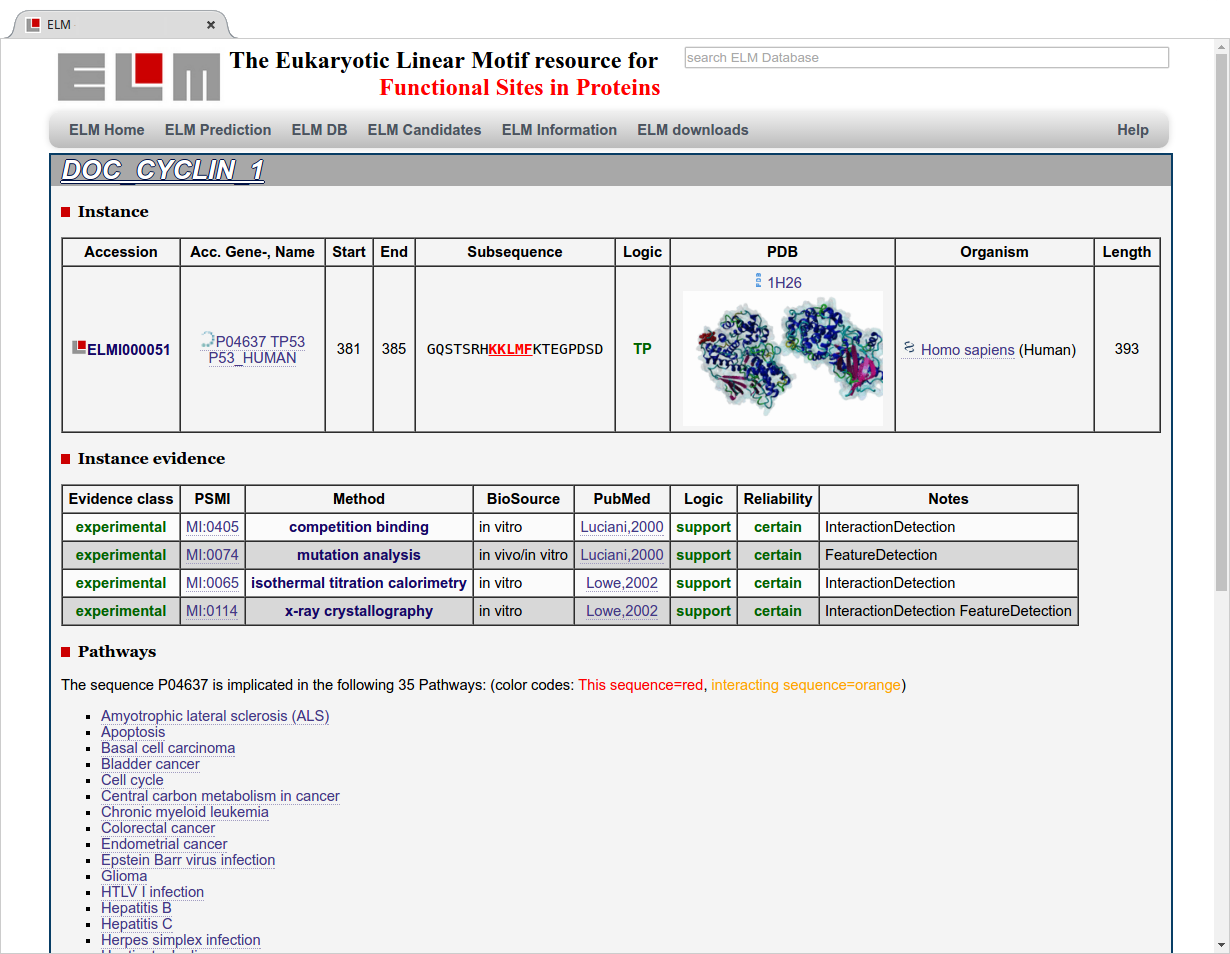
\includegraphics[width=\textwidth]{Figures/explore_content/doc_cyclin_1_instance.png}
	\caption{
	The instance details page for the \motif{DOC\_CYCLIN\_1} instance annotated
	for protein \uniprot{P53\_HUMAN} with start/end position ``381-385''. This page
	also contains links to many external databases including Uniprot
	\cite{25348405}, PDB \cite{12037327}, NCBI taxonomy, Pubmed
	\cite{27899561}, and KEGG Pathways \cite{26476454}, as well as the
	PSI-MI controlled vocabulary \cite{17925023}.
	}
	\label{fig:explore_content_doc_cyclin_instance}
\end{figure}

\item Type ``p53\_human'' in the search box to search for ELM Instances in this
	protein. Find the row for the ELM class \motif{DOC\_CYCLIN\_1} and click on
	the instance subsequence (highlighted in red) to go to the instance
	details page of this
	instance (Fig. \ref{fig:explore_content_doc_cyclin_instance})
	The top part of the page contains details about the instance
	and the protein it was identified in, and link to the Uniprot entry for
	the protein \cite{25348405}.

\item Scroll down to the ``Instance Evidence'' header to view details on the
	experimental evidence used to annotate this instance. The each
	experimental method is annotated using the Proteomics Standards
	Initiative Method Identifier (PSI-MI) \cite{17925023} as well as the
	references in which the experiments were published.

	\sdesc{
		The ``biosource'' indicates whether method is \textit{in vivo},
		\textit{in vitro}, \textit{in sicilo} or a combination of these.
		The ``logic'' column indicates whether this experiment
		``supports'' or ``contradicts'' this instance being functional.
		Each method is also annotated with a ``reliability'', which can
		be any of ``certain'', ``likely'', ``unlikely'' or
		``unspecified''.}

%
% Subsection: Switches, pathways and other external resources. 
%
\subsection{Finding Switches and molecular interactions}
\label{subsec:explore_content_external_resoureces}

\begin{figure}[h!]
	\centering
	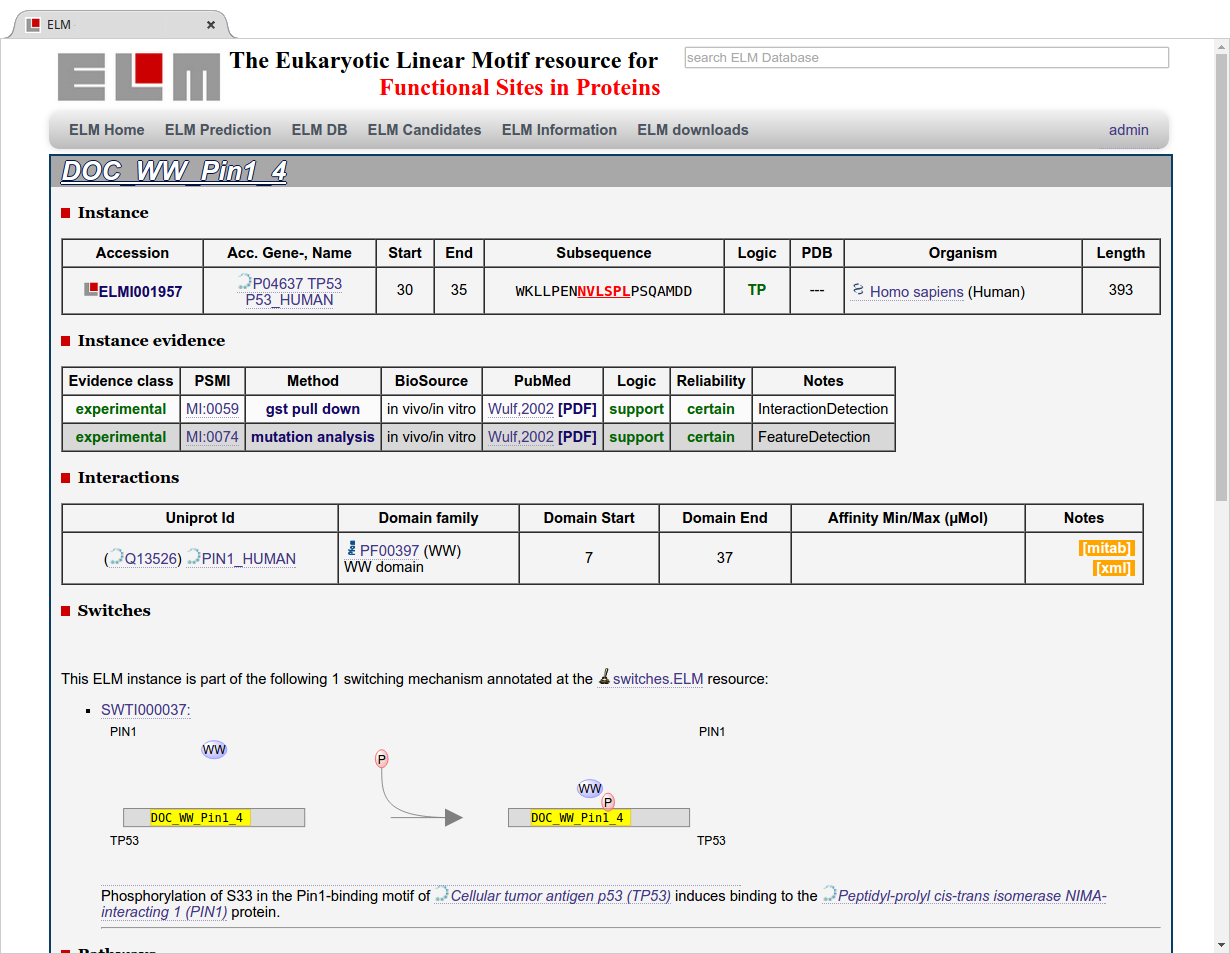
\includegraphics[width=\textwidth]{Figures/explore_content/doc_ww_pin_1_4_instance.png}
	\caption{
	The instance details page for the \motif{DOC\_WW\_Pin1\_4}
	instance found in Human P53 (\uniprot{P53\_HUMAN}) with start/end position
	``30-35''.
	}
	\label{fig:explore_content_doc_ww_instance}
\end{figure}

\item Repeat the previous search by clicking on the sub-menu \button{ELM instances}
	under \button{ELM DB} and type ``p53\_human'' in the search box. This time,
	find the ELM instance \motif{DOC\_WW\_Pin1\_4} motif with the
	start/end position ``30-35''. (You can sort the table by clicking on the
	header lines: click on ``Start'' to sort by start position ). Click on the
	start/end position or the subsequence which will take you to the details
	page (Fig. \ref{fig:explore_content_doc_ww_instance}). This
	page is similar to that described for the P53 instance \motif{DOC\_CYCLIN\_1}
	(Fig. \ref{fig:explore_content_doc_cyclin_instance}).
	Additionally, for this instance there is information available about
	its interaction partner and a molecular switch which is mediated by
	this motif instance.

\item Scroll down to the ``Interactions'' header to view information about this
	instance's interactions
	(Fig.  \ref{fig:explore_content_doc_ww_instance}). This instance
	interacts with \uniprot{PIN1\_Human} via the ``WW'' domain (Pfam identifier
	PF00397; found on position 7-37 in \uniprot{PIN1\_Human}. If available,
	binding affinities are also shown here. Interaction data is made
	available in \fileformat{mitab} and \fileformat{xml} format
	(\cite{17925023}), and can be downloaded by clicking on the yellow
	buttons in the right column.

\item Scroll further down to the ``Switches'' section for a brief overview of
	the switches details of this instance obtained form switches.ELM
	(\cite{23550212}) (Fig. \ref{fig:explore_content_doc_ww_instance}). This
	particular instance is involved in the switch phosphorylating P53.
	Clicking on the diagram will open an external link to the
	switches.ELM website.

%
% Subsection: Links to external resources
%
\subsection{Exploring Links External Protein Resources}
\label{subsec:explore_content_links_to_external_resources}

\begin{figure}[h!]
	\centering
	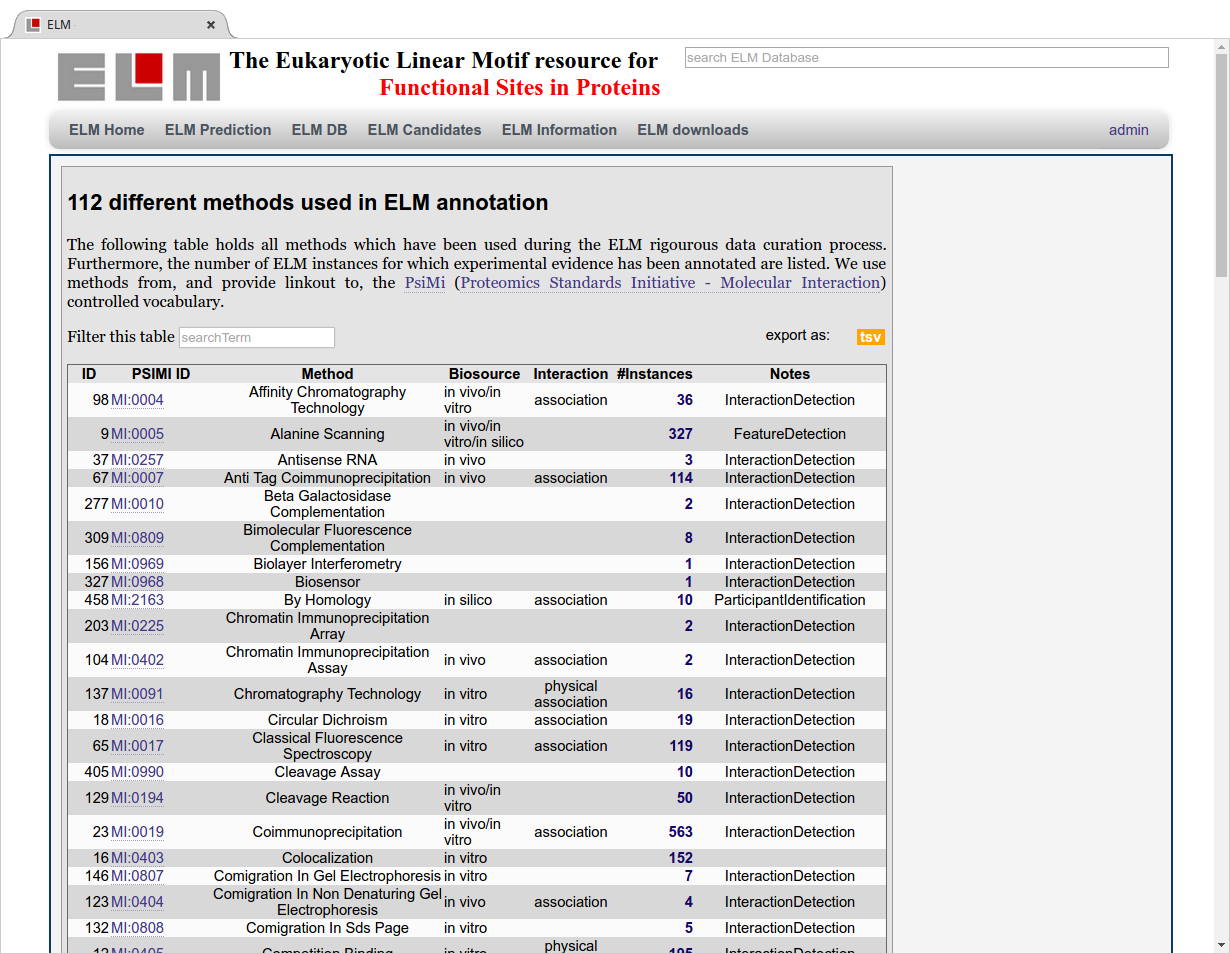
\includegraphics[width=\textwidth]{Figures/explore_content/methods.png} 
	\caption{
		The list of all experimental methods used in the ELM database,
		along with their PSI-MI identifiers.
	}
	\label{fig:explore_content_methods}
\end{figure}

\item Click on the sub-menu \button{ELM methods} in \button{ELM DB} to see a
	list of all experimental methods which have been used to identify
	motifs and instances
	(Fig \ref{fig:explore_content_methods}).
	This table shows the internal method
	identifier in the first column, a link to the corresponding entry in
	the PSI-MI database (\cite{17925023}), and the method name as annotated
	by the PSI-MI controlled vocabulary, as well as the type of experiment
	(in vitro/in vivo). Clicking on the link in the ``instances'' column
	will list all instances annotated using that method.  

	\sdesc{The filter bar on the top page can be used to filter the list of
		methods. The \fileformat{tsv} link creates a downloadable file
		in ``tab separated values'' format.}

\begin{figure}[h!]
	\centering
	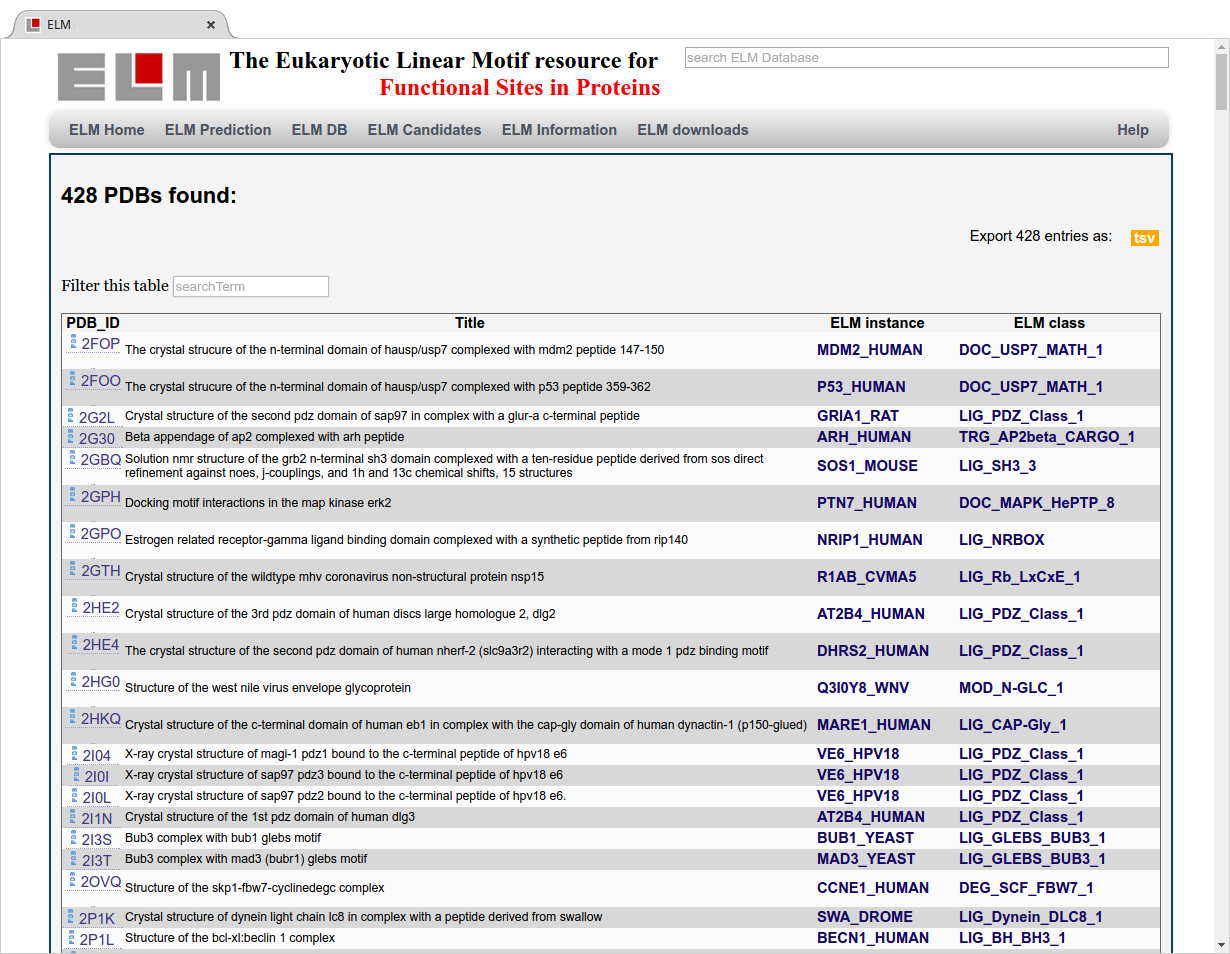
\includegraphics[width=\textwidth]{Figures/explore_content/pdbs.png} 
	\caption{
	The list of all known structures in PDB which are also in ELM.
	}
	\label{fig:explore_content_pdbs}
\end{figure}

\item Click on the sub-menu \button{ELM pdb structures} in \button{ELM DB} to
	see a list of all macromolecular structures in the ELM database
	(Fig. \ref{fig:explore_content_pdbs}).
	Structures annotated in ELM ideally (but not always) show
	both interaction partners, motif and domain. This page also contains
	links to RCSB/PDB (\cite{12037327}), the individual instance and the motif
	class of that instance.

	\sdesc{The filter bar on the top page can be used to filter the list of
		structures shown. The yellow \fileformat{tsv} link creates a
		downloadable file in ``tab separated values'' format.}

\begin{figure}[h!]
	\centering
	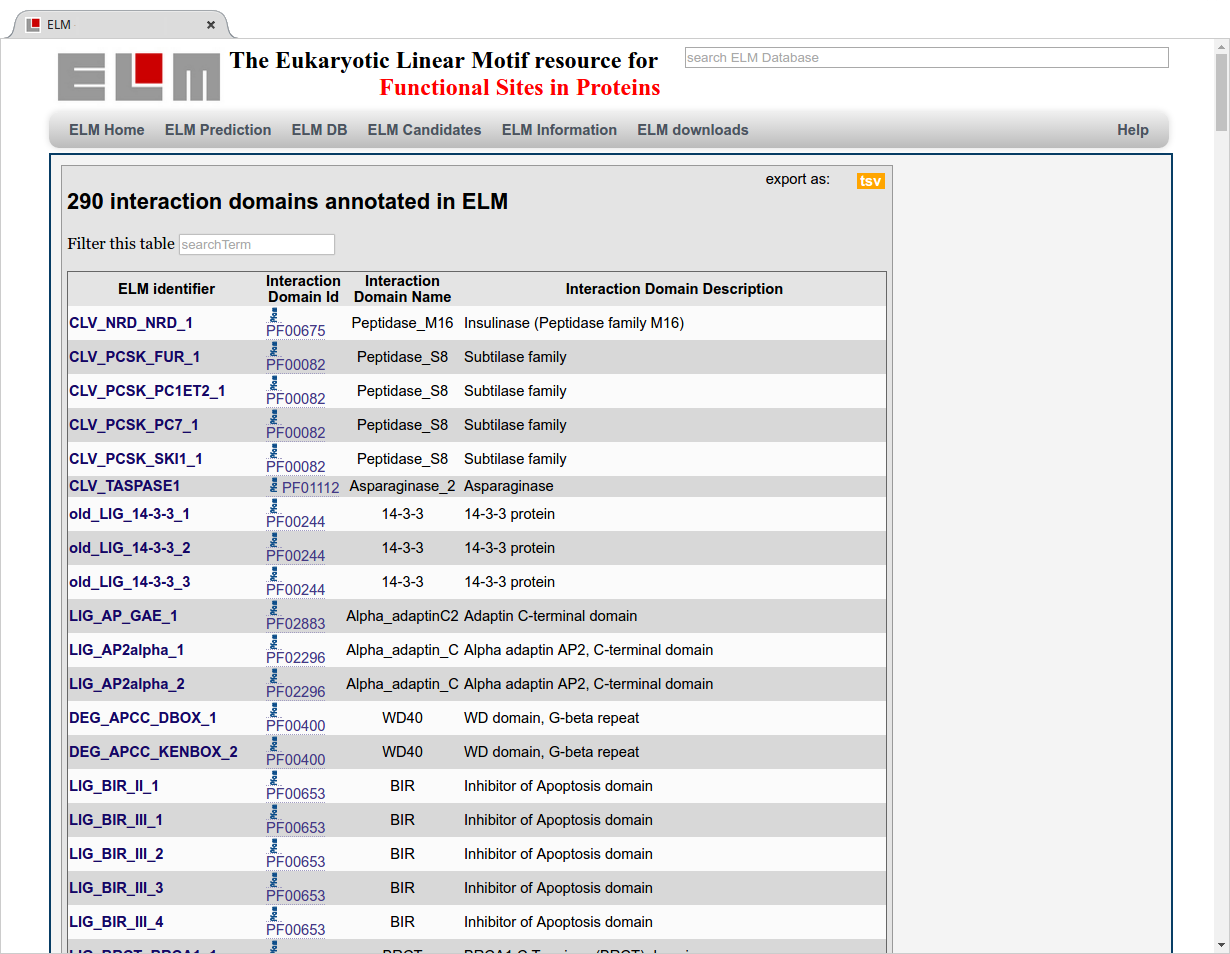
\includegraphics[width=\textwidth]{Figures/explore_content/interactiondomains.png}
	\caption{
	A list of all interactions annotated in the database.
	}
	\label{fig:explore_content_interaction_domains}
\end{figure}

\item Click on the sub-menu \button{ELM binding domains} under \button{ELM DB}
	to see a complete list of all the interaction domains in ELM
	(Fig. \ref{fig:explore_content_interaction_domains}).
	This table shows the ELM classes which have been annotated
	with a corresponding interaction domain. This table shows the ELM
	class, a link to the Pfam \cite{26673716}, SMART \cite{25300481} or 
	InterPro (\cite{27899635}) domain, as well as the name of the
	interacting domain followed by a brief description.

	\sdesc{The filter bar on the top page can be used to filter the list of
		interactions shown. The \emph{tsv} link creates a downloadable
		file in ``tab separated values'' format.}

%
\begin{figure}[h!]
	\centering
	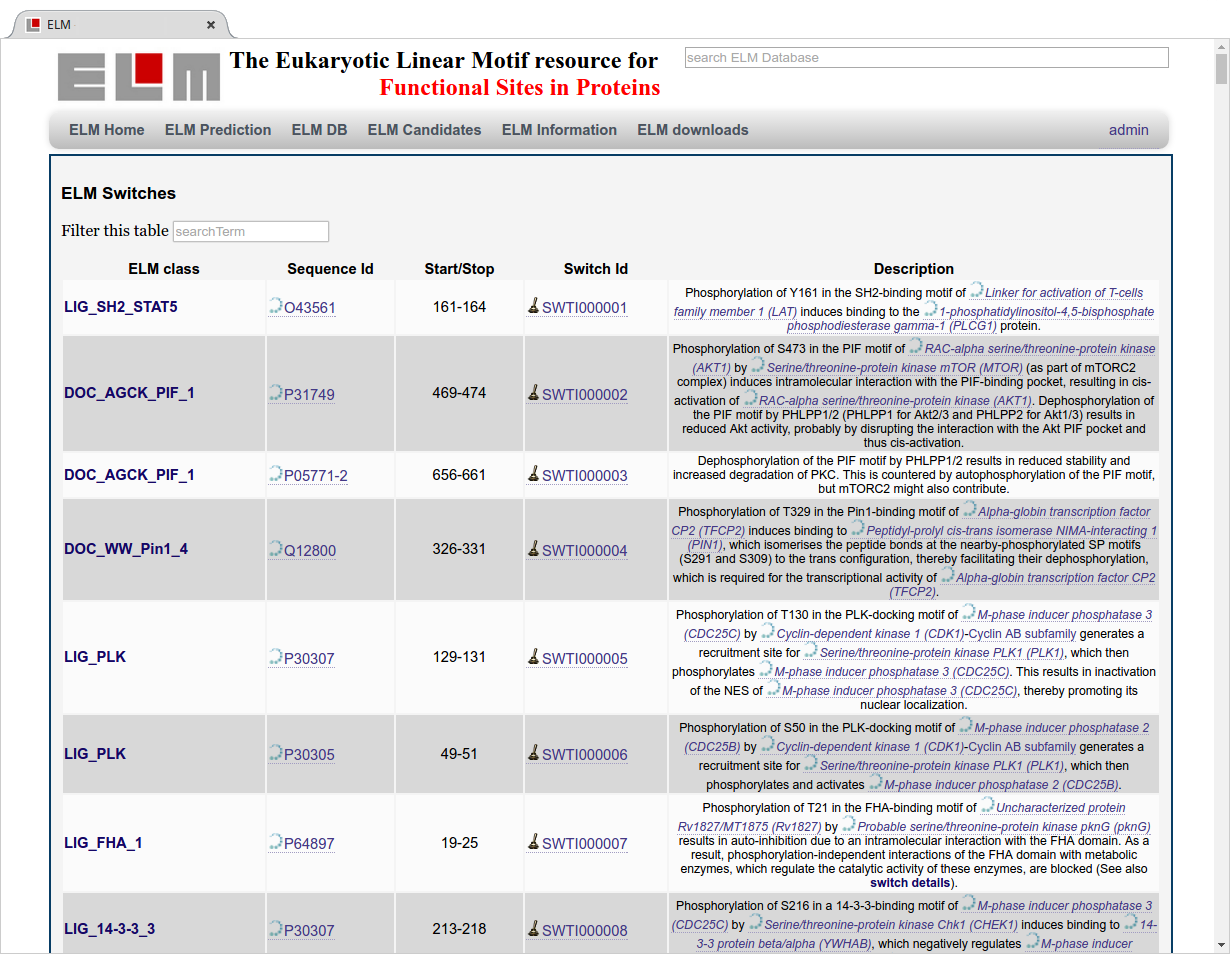
\includegraphics[width=\textwidth]{Figures/explore_content/switches.png} 
	\caption{
		A list of all switches annotated switches.ELM also contained in ELM.
	}
	\label{fig:explore_content_switches}
\end{figure}

\item Click on the sub-menu \button{ELM switches} in \button{ELM DB} to see a complete
	list of all the switches in ELM
	(Fig. \ref{fig:explore_content_switches}). This table shows
	the motif class, contains a link to Uniprot, and the start and stop
	positions of the motif mediating the switch. The last two columns have
	links to switches.ELM, and a brief description of the switch also taken
	from switches.ELM \cite{23550212}.

	\sdesc{The filter bar on the top page can be used to quickly filter
		the list of interactions shown.} 

%
% Subsection: Exploreing KEGG pathways
%

\subsection{Visualizing KEGG pathways from ELM}
\label{subsec:explore_content_kegg}

\begin{figure}[h!]
	\centering
	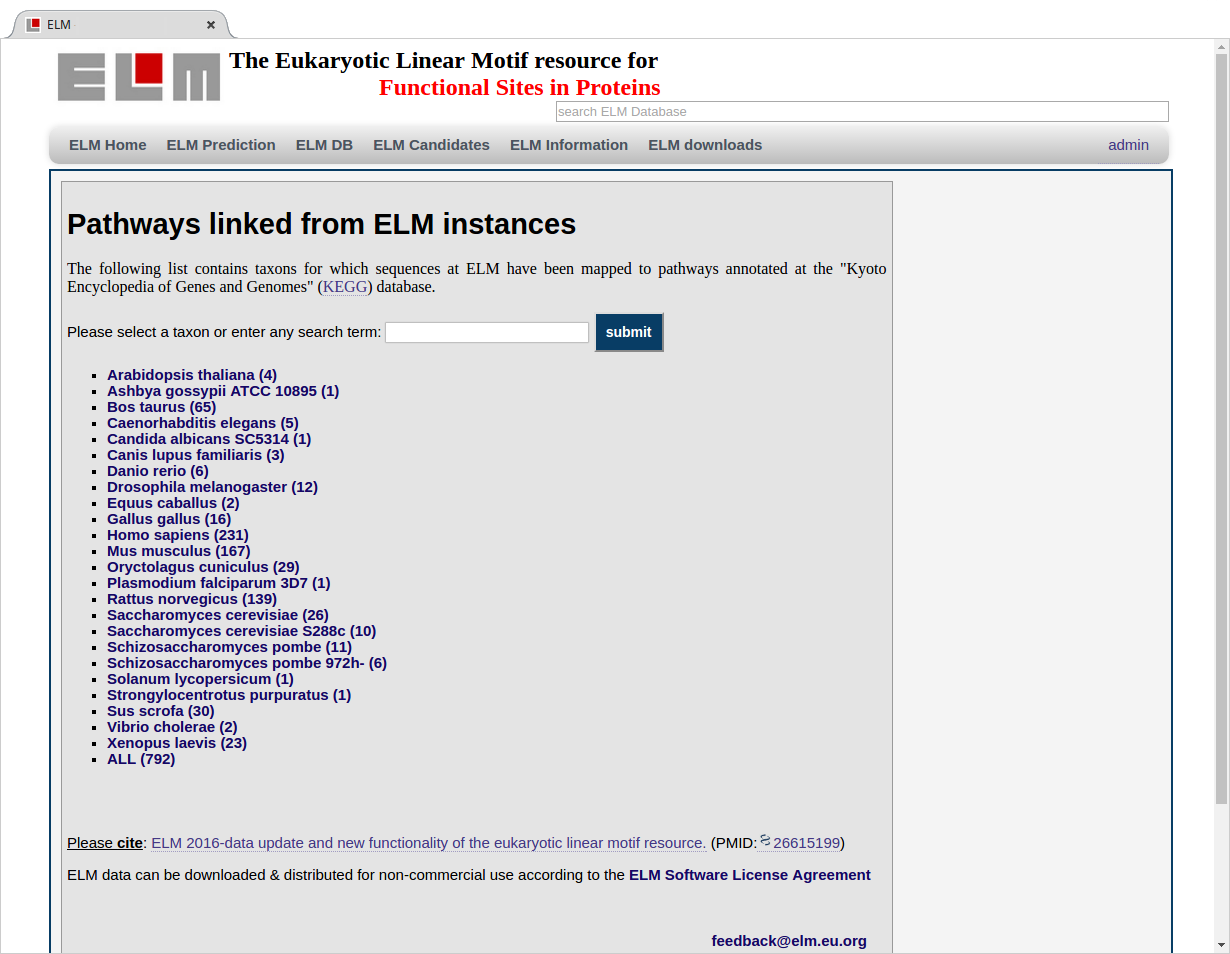
\includegraphics[width=\textwidth]{Figures/explore_content/pathways.png} 
	\caption{
	A list of all Pathways from KEGG with proteins in ELM.
	}
	\label{fig:explore_content_pathways}
\end{figure}

\item Click on the sub-menu \button{ELM pathways} in \button{ELM DB} to see a list of all
	KEGG pathways contained in ELM
	(Fig. \ref{fig:explore_content_pathways}).
	Pathways are from the ``Kyoto Encyclopedia of Genes and Genomes'' (KEGG
	\cite{26476454}) database mapped to ELM instances. 
	
\begin{figure}[h!]
	\centering
	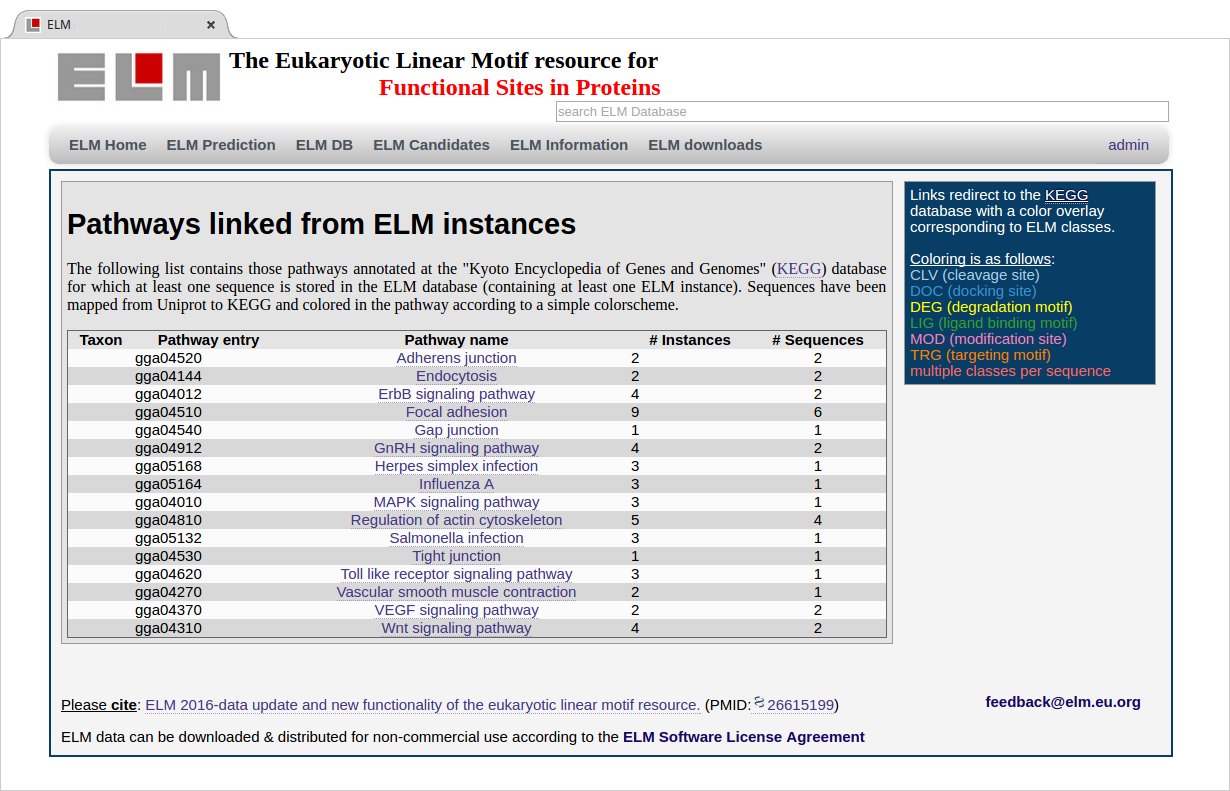
\includegraphics[width=\textwidth]{Figures/explore_content/pathways_example.png} 
	\caption{
		A list of all KEGG pathways in \textit{Gallus gallus} involving proteins annotated in ELM.
	}
	\label{fig:explore_content_pathways_example}
\end{figure}

\item On the ``ELM pathways'' page
	(Fig.  \ref{fig:explore_content_pathways_example})
	click on the link \button{gallus gallus} to navigate to the page
	containing all pathways annotated for
	chicken.

\begin{figure}[h!]
	\centering
	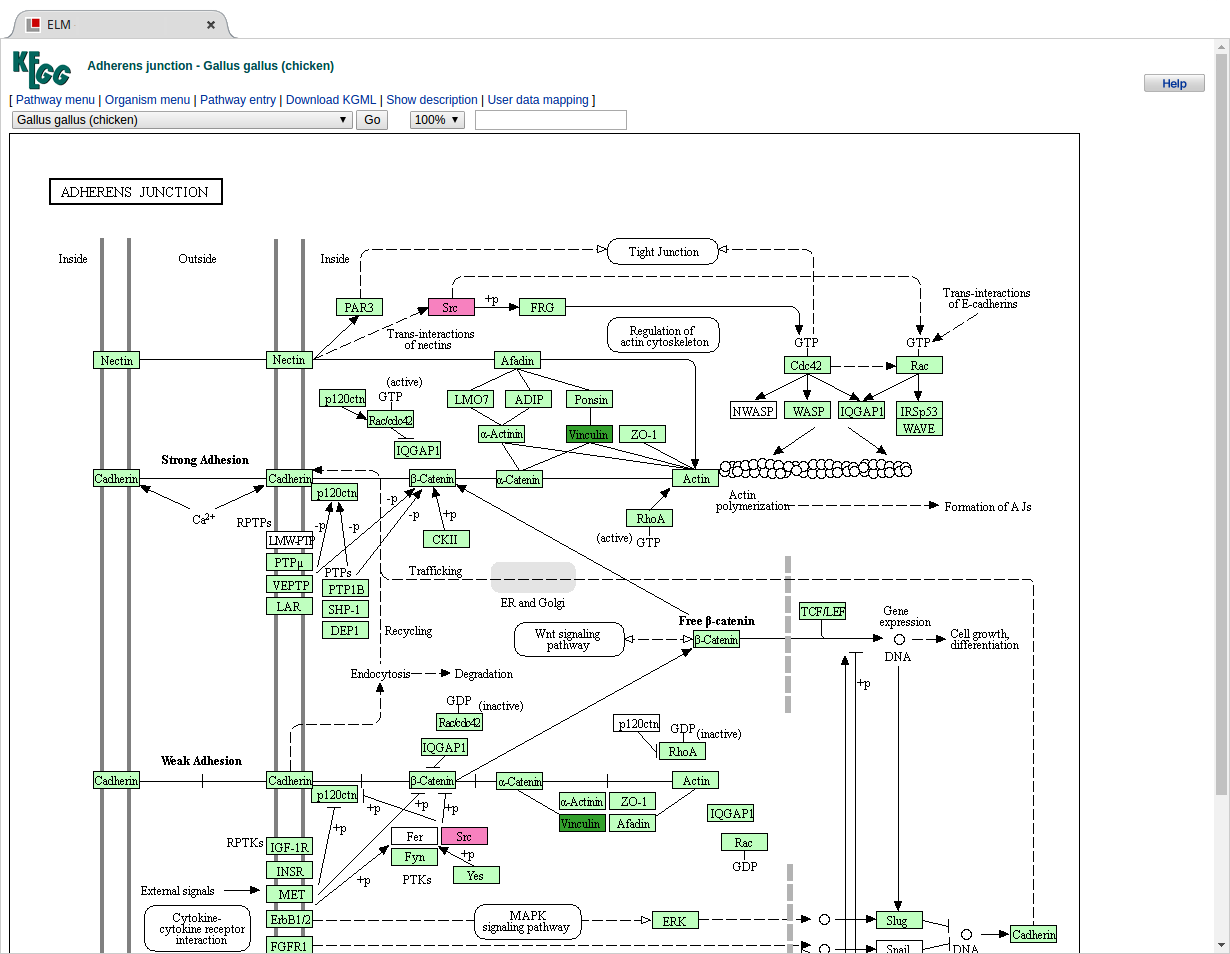
\includegraphics[width=\textwidth]{Figures/explore_content/pathways_kegg.png} 
	\caption{
	A list of all annotated pathways for taxon \textit{Gallus gallus}
	}
	\label{fig:explore_content_pathways_kegg}
\end{figure}

\item One the page with chicken pathways
	(Fig. \ref{fig:explore_content_pathways_example})
	click on \button{Adherens junction} to the KEGG entry for this pathway,
	with each protein's color corresponding to ELM classes (see the color
	legend right side of figure \ref{fig:explore_content_pathways_kegg}).

%
% Subsection: Infections and Diseases
%
\subsection{Browsing Infections and Diseases}
\label{subsec:explore_content_infections_and_diseases}

\begin{figure}[h!]
	\centering
	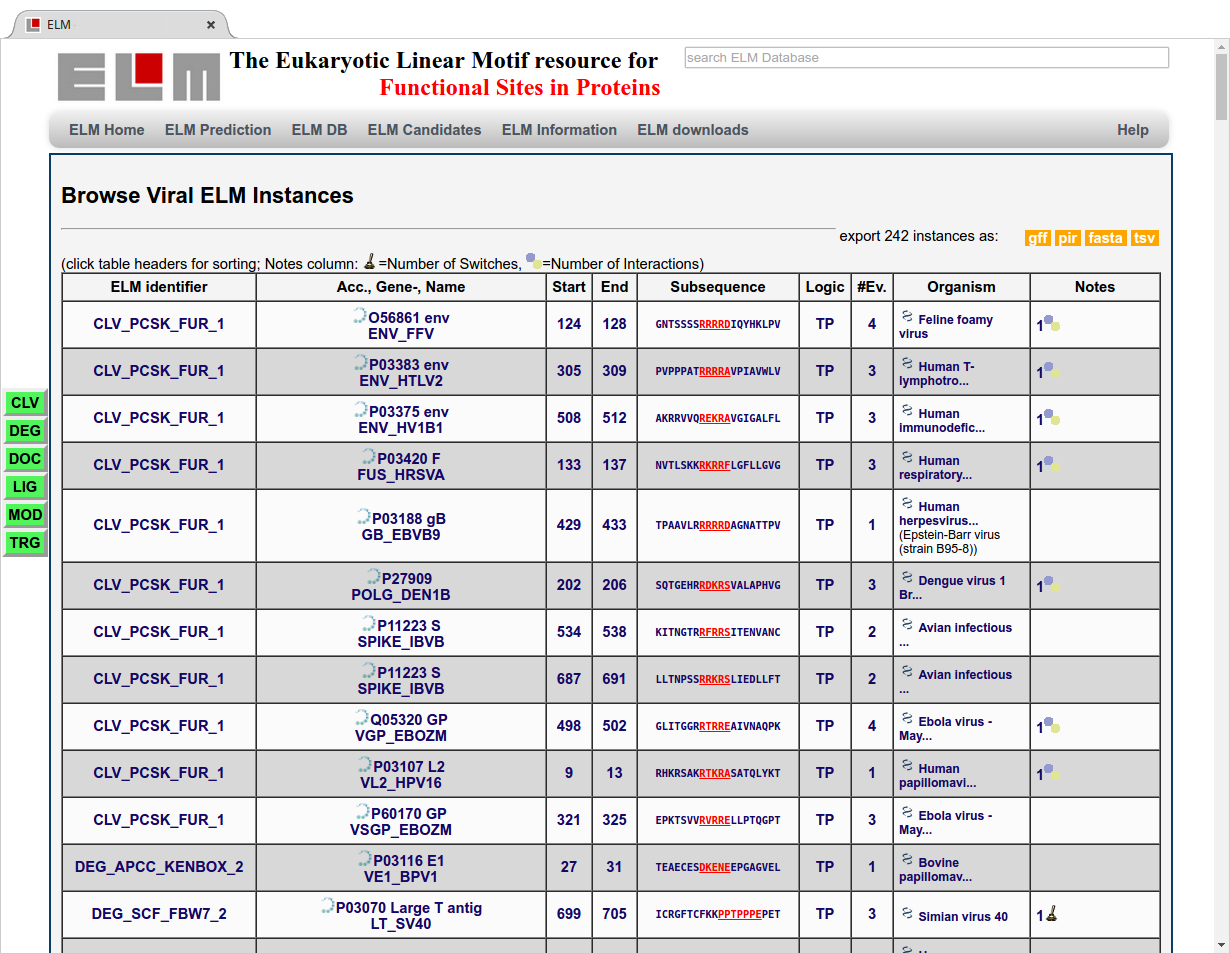
\includegraphics[width=\textwidth]{Figures/explore_content/viruses.png} 
	\caption{
		A table of the ELM instances abused by viruses.
	}
	\label{fig:explore_content_viruses}
\end{figure}

\item Click on the sub-menu \button{ELM virus instances} under \button{ELM DB}
	to see a list of all instances in ELM that have been annotated as being
	abused by viruses (Fig. \ref{fig:explore_content_viruses}).
	The columns are identical to those listed in Step 7 (Fig.  
	\ref{fig:explore_content_instances}).

	\sdesc{The green buttons on the left can be used to filter this table
		by motif class. Click on the yellow links on the top right of
		the page to download the (complete) table in \fileformat{gff},
		\fileformat{pir}, \fileformat{fasta} or \fileformat{tsv}
		format.}

\begin{figure}[h!]
	\centering
	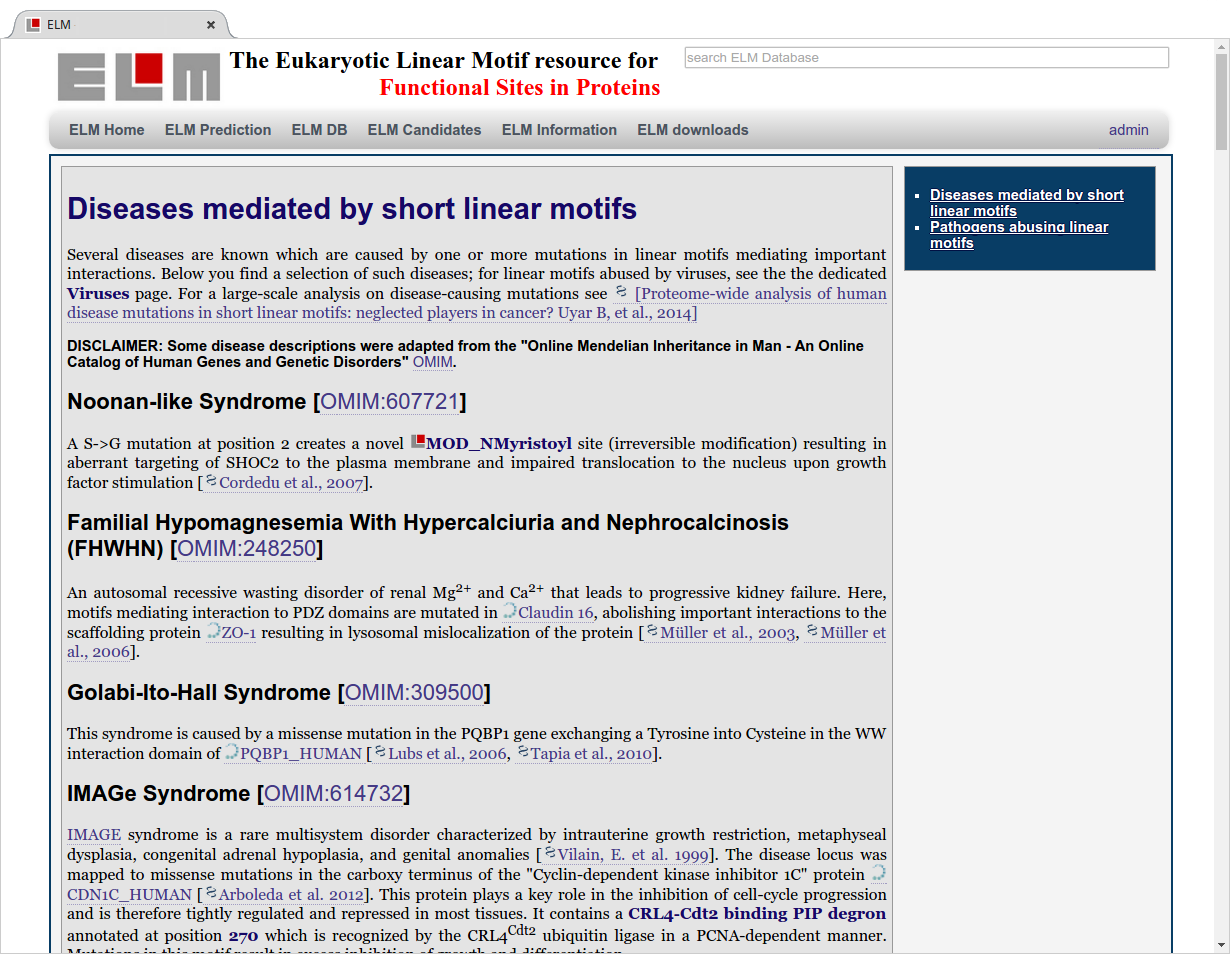
\includegraphics[width=\textwidth]{Figures/explore_content/diseases.png}
	\caption{
	A list of all diseases in ELM.
	}
	\label{fig:explore_content_diseases}
\end{figure}

\item Click on the sub-menu \button{ELM diseases} under \button{ELM DB} to see
	a list of all motif classes that have been annotated with a disease
	(Fig. \ref{fig:explore_content_diseases}). Disease information is taken
	from the Online Mendelian Inheritance in Man (OMIM) database
	\cite{17357067}.

%
% Subsection: Help page 
%
\subsection{Finding Help and Frequently Asked Questions}
\label{subsec:explore_content_help}

\begin{figure}[h!]
	\centering
	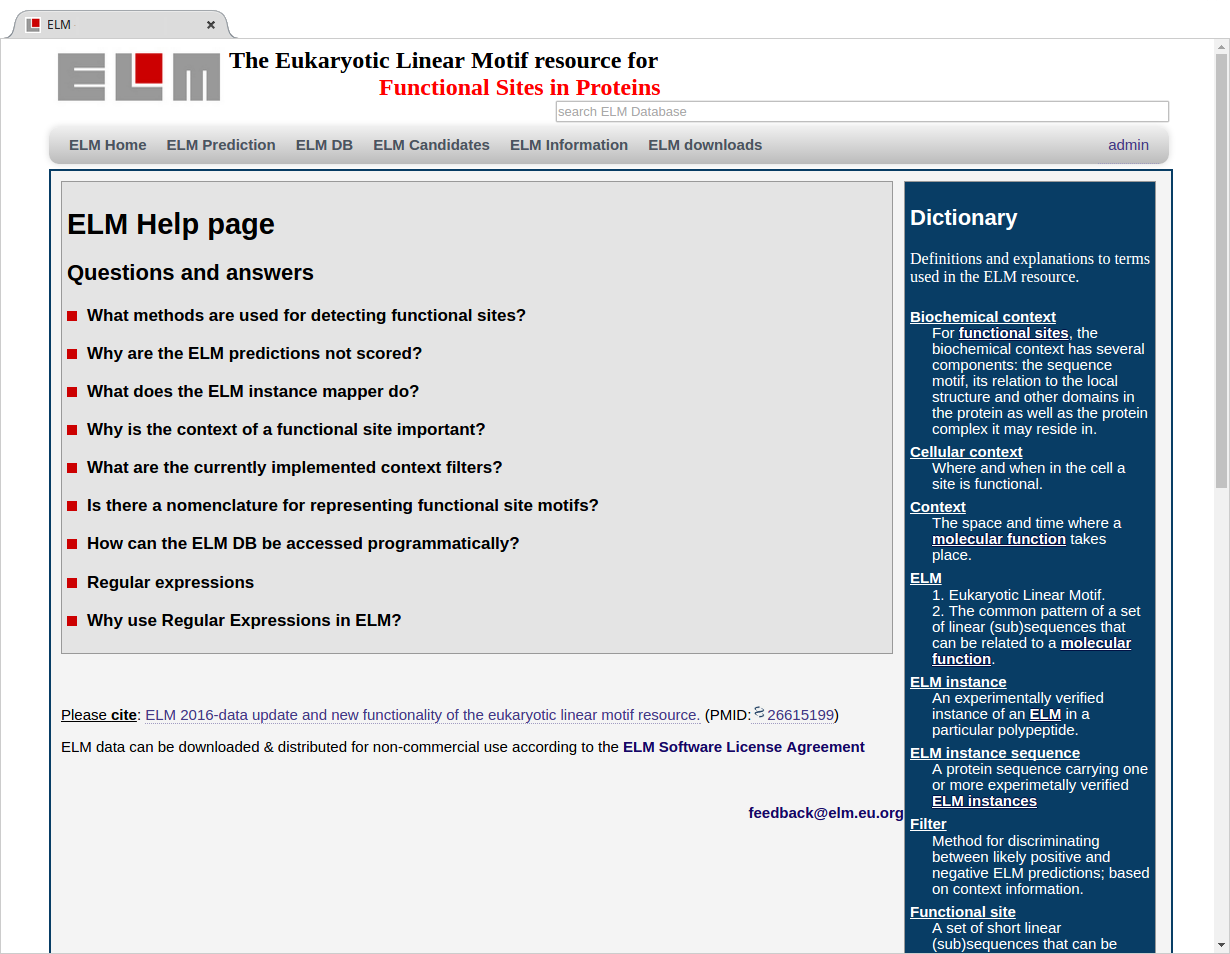
\includegraphics[width=\textwidth]{Figures/explore_content/help.png} 
	\caption{
		The ELM help and Questions \& Answers page.
	}
	\label{fig:explore_content_viruses}
\end{figure}

\item Click on the \button{Help} button on the right of the top navigation menu
	to visit the ELM Help page. This page has answers to the most
	Frequently asked questions, which you can see by clicking on a
	particular question. For example: Click on ``Regular expressions'' for
	a detailed description of the symbols used to build regular expressions
	to define motif classes.
\end{enumerate}

